\section{Classes}
There are a grand total of 21 classes in the Elder Scrolls Tabletop RPG, each with a unique combination of favored skills and attributes. You may wish to become more acquainted with what the skills mean in order to make an informed decision about which class you choose.\\

A class consists of 4 components:
\begin{enumerate}
	\item A name.
	\item A specialization (combat, magic or stealth).
	\item Two favored primary attributes.
	\item Seven major skills.
\end{enumerate}

All skills grouped under the chosen specialization get a +5 bonus. The two favored attributes gain a +5 bonus as well. The seven major skills gain a +20 bonus; the remaining 14 skills are defined as minor skills. If you wish to create a custom class, simply choose the four components on your own. You should look over the 21 existing classes, however -- odds are you'll find multiple appealing choices.\\

\begin{longtable}{lm{0.6\textwidth}}
	\raisebox{-0.5\height}{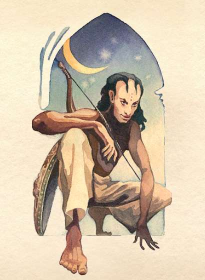
\includegraphics[width=0.3\textwidth]{classes/acrobat.png}} & 
\textbf{\Large Acrobat}\newline

The kind of person that uses agility and endurance to their advantage. Unafraid of jumping long distances.\newline

\textbf{Specialization}: Stealth\newline
\textbf{Attributes}: Agility, Endurance\newline
\textbf{Skills}: Acrobatics, Blade, Block, Marksman, Security, Sneak, Speechcraft\\

	\raisebox{-0.5\height}{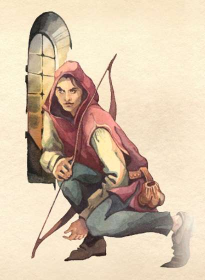
\includegraphics[width=0.3\textwidth]{classes/agent.png}} & \textbf{\Large Agent}\newline

Charming when they can be seen, and nearly invisible when in shadow.\newline

\textbf{Specialization}: Stealth\newline
\textbf{Attributes}: Agility, Personality\newline
\textbf{Skills}: Acrobatics, Illusion, Marksman, Mercantile, Security, Sneak, Speechcraft\\

	\raisebox{-0.5\height}{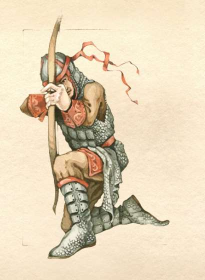
\includegraphics[width=0.3\textwidth]{classes/archer.png}} & \textbf{\Large Archer}\newline

A marksman, adept at combat at great distances. Able to take down most foes before they have a chance to draw sword.\newline

\textbf{Specialization}: Combat\newline
\textbf{Attributes}: Agility, Strength\newline
\textbf{Skills}: Armorer, Blade, Blunt, Hand-to-Hand, Light Armor, Marksman, Sneak\\

	\raisebox{-0.5\height}{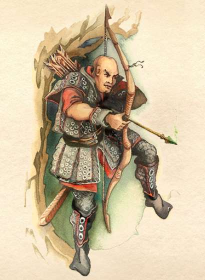
\includegraphics[width=0.3\textwidth]{classes/assassin.png}} & \textbf{\Large Assassin}\newline

Nimble and quiet, they move in darkness to strike at the unsuspecting. Locks hold no doors shut for them.\newline

\textbf{Specialization}: Stealth\newline
\textbf{Attributes}: Intelligence, Speed\newline
\textbf{Skills}: Acrobatics, Alchemy, Blade, Light Armor, Marksman, Security, Sneak\\

	\raisebox{-0.5\height}{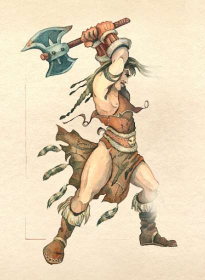
\includegraphics[width=0.3\textwidth]{classes/barbarian.png}} & \textbf{\Large Barbarian}\newline

Fearsome brutes who inspire fear and dread in the hearts of their enemies. Like a storm, swift and powerful. Finding little use for heavy armor, they rely on smashing their foes into the ground.\newline

\textbf{Specialization}: Combat\newline
\textbf{Attributes}: Speed, Strength\newline
\textbf{Skills}: Armorer, Athletics, Blade, Block, Blunt, Hand-to-Hand, Light Armor\\

	\raisebox{-0.5\height}{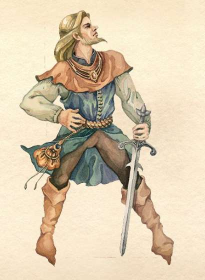
\includegraphics[width=0.3\textwidth]{classes/bard.png}} & \textbf{\Large Bard}\newline

Intelligent and personable, they prefer to accomplish tasks with their words first, and sword second.\newline

\textbf{Specialization}: Stealth\newline
\textbf{Attributes}: Intelligence, Personality\newline
\textbf{Skills}: Alchemy, Blade, Block, Illusion, Light Armor, Mercantile, Speechcraft\\

	\raisebox{-0.5\height}{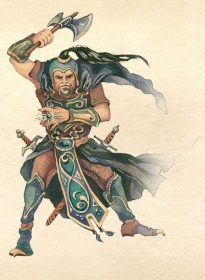
\includegraphics[width=0.3\textwidth]{classes/battlemage.png}} & \textbf{\Large Battlemage}\newline

Able to resolve most conflicts with either spell or sword. They are a deadly mix of scholar and soldier.\newline

\textbf{Specialization}: Magic\newline
\textbf{Attributes}: Intelligence, Strength\newline
\textbf{Skills}: Alchemy, Alteration, Blade, Blunt, Conjuration, Destruction, Mysticism\\

	\raisebox{-0.5\height}{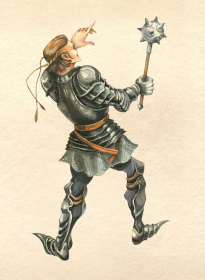
\includegraphics[width=0.3\textwidth]{classes/crusader.png}} & \textbf{\Large Crusader}\newline

A combatant who wields the power of brute strength and medicinal knowledge. Cheating death after every fight, they rely on their keen knowledge of restoration to fight yet again.\newline

\textbf{Specialization}: Combat\newline
\textbf{Attributes}: Strength, Willpower\newline
\textbf{Skills}: Athletics, Blade, Blunt, Destruction, Hand-to-Hand, Heavy Armor, Restoration\\

	\raisebox{-0.5\height}{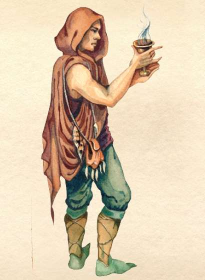
\includegraphics[width=0.3\textwidth]{classes/healer.png}} & \textbf{\Large Healer}\newline

Fighters of poison and illness. The ancient art of restoration is their ally, and the deadly art of destruction is their weapon.\newline

\textbf{Specialization}: Magic\newline
\textbf{Attributes}: Personality, Willpower\newline
\textbf{Skills}: Alchemy, Alteration, Destruction, Illusion, Mercantile, Restoration, Speechcraft\\

\raisebox{-0.5\height}{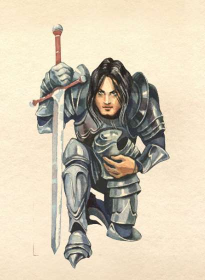
\includegraphics[width=0.3\textwidth]{classes/knight.png}} & \textbf{\Large Knight}\newline

The most noble of all combatants. Strong in body and in character.\newline

\textbf{Specialization}: Combat\newline
\textbf{Attributes}: Personality, Strength\newline
\textbf{Skills}: Blade, Block, Blunt, Hand-to-Hand, Heavy Armor, Illusion, Speechcraft\\

	\raisebox{-0.5\height}{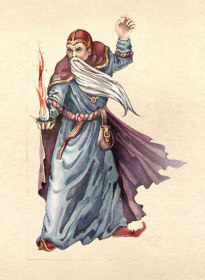
\includegraphics[width=0.3\textwidth]{classes/mage.png}} & \textbf{\Large Mage}\newline

Preferring to use their extensive knowledge of all things magical, they wield a might more powerful than the sharpest blade.\newline

\textbf{Specialization}: Magic\newline
\textbf{Attributes}: Intelligence, Willpower\newline
\textbf{Skills}: Alchemy, Alteration, Conjuration, Destruction, Illusion, Mysticism, Restoration\\

\raisebox{-0.5\height}{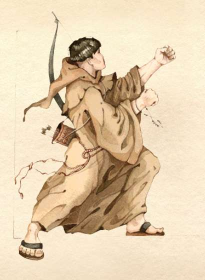
\includegraphics[width=0.3\textwidth]{classes/monk.png}} & \textbf{\Large Monk}\newline

Quick and cunning with the empty hand, they are strong in spirit. They prefer to solve conflict by arrow or by fist.\newline

\textbf{Specialization}: Stealth\newline
\textbf{Attributes}: Agility, Willpower\newline
\textbf{Skills}: Acrobatics, Alteration, Athletics, Hand-to-Hand, Marksman, Security, Sneak\\

\raisebox{-0.5\height}{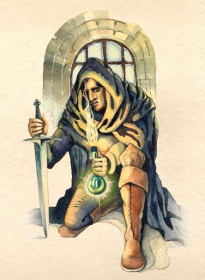
\includegraphics[width=0.3\textwidth]{classes/nightblade.png}} & \textbf{\Large Nightblade}\newline

Spell and shadow are their friends. By darkness they move with haste, casting magic to benefit their circumstances.\newline

\textbf{Specialization}: Magic\newline
\textbf{Attributes}: Speed, Willpower\newline
\textbf{Skills}: Acrobatics, Alteration, Athletics, Blade, Destruction, Light Armor, Restoration\\

\raisebox{-0.5\height}{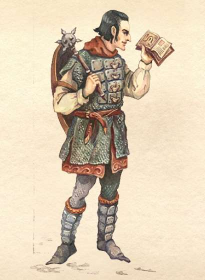
\includegraphics[width=0.3\textwidth]{classes/pilgrim.png}} & \textbf{\Large Pilgrim}\newline

Hearty folk, well-versed in the tomes of old. They profit in life by bartering in the market, or by persuading the weak-minded.\newline

\textbf{Specialization}: Stealth\newline
\textbf{Attributes}: Endurance, Personality\newline
\textbf{Skills}: Armorer, Block, Blunt, Light Armor, Mercantile, Security, Speechcraft\\

	\raisebox{-0.5\height}{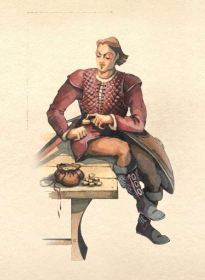
\includegraphics[width=0.3\textwidth]{classes/rogue.png}} &
\textbf{\Large Rogue}\newline

They use speed in combat rather than brute force. Persuasive in conversation, their tongues are as sharp as blades.\newline

\textbf{Specialization}: Combat\newline
\textbf{Attributes}: Personality, Speed\newline
\textbf{Skills}: Alchemy, Athletics, Blade, Block, Illusion, Light Armor, Mercantile\\


	\raisebox{-0.5\height}{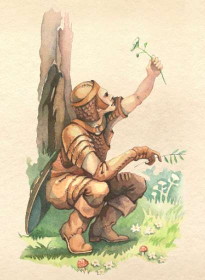
\includegraphics[width=0.3\textwidth]{classes/scout.png}} &
\textbf{\Large Scout}\newline

Preferring the rolling countryside to the city life, they are gifted with the ability to evade, guard and protect themselves with great proficiency.\newline

\textbf{Specialization}: Combat\newline
\textbf{Attributes}: Endurance, Speed\newline
\textbf{Skills}: Acrobatics, Alchemy, Armorer, Athletics, Blade, Block, Light Armor\\

	\raisebox{-0.5\height}{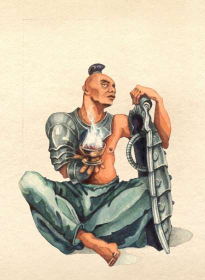
\includegraphics[width=0.3\textwidth]{classes/sorcerer.png}} & \textbf{\Large Sorcerer}\newline

Besting the most well-equipped fighters, they rely on the spells of the mystic arts. Unique to these mages is the bodily stamina to be armed with the thickest armor.\newline

\textbf{Specialization}: Magic\newline
\textbf{Attributes}: Endurance, Intelligence\newline
\textbf{Skills}: Alchemy, Alteration, Conjuration, Destruction, Heavy Armor, Mysticism, Restoration\\

	\raisebox{-0.5\height}{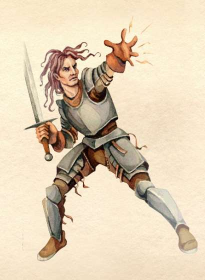
\includegraphics[width=0.3\textwidth]{classes/spellsword.png}} & \textbf{\Large Spellsword}\newline

More nimble and athletic than the sorcerer, and better suited for spell-casting than the knight, their attacks are unpredictable. Students of combat and magic.\newline

\textbf{Specialization}: Magic\newline
\textbf{Attributes}: Endurance, Willpower\newline
\textbf{Skills}: Alteration, Blade, Block, Heavy Armor, Destruction, Illusion, Restoration\\

	\raisebox{-0.5\height}{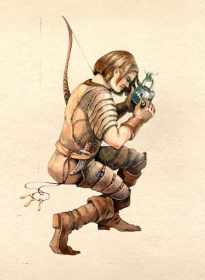
\includegraphics[width=0.3\textwidth]{classes/thief.png}} & \textbf{\Large Thief}\newline

Profiting from the losses of others is their love. Able to be swift in shadow, and crafty in bartering. Locks are enemies, and lock-picks are their swords.\newline

\textbf{Specialization}: Stealth\newline
\textbf{Attributes}: Agility, Speed\newline
\textbf{Skills}: Acrobatics, Light Armor, Marksman, Mercantile, Security, Sneak, Speechcraft\\

	\raisebox{-0.5\height}{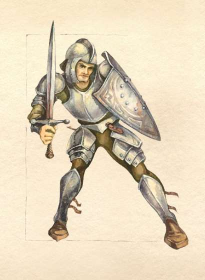
\includegraphics[width=0.3\textwidth]{classes/warrior.png}} & \textbf{\Large Warrior}\newline

Unafraid of light weaponry, they plow into the fray with little regard for injury. Masters of all melee tools, they put little faith in the magical arts.\newline

\textbf{Specialization}: Combat\newline
\textbf{Attributes}: Endurance, Strength\newline
\textbf{Skills}: Armorer, Athletics, Blade, Block, Blunt, Hand-to-Hand, Heavy Armor\\

	\raisebox{-0.5\height}{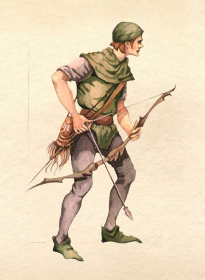
\includegraphics[width=0.3\textwidth]{classes/witchhunter.png}} & \textbf{\Large Witchhunter}\newline

Swift on foot, and clever with spells, they use distance as their ally. Slower adversaries are fodder for their arrows.\newline

\textbf{Specialization}: Magic\newline
\textbf{Attributes}: Agility, Intelligence\newline
\textbf{Skills}: Alchemy, Athletics, Conjuration, Destruction, Marksman, Mysticism, Security\\
\end{longtable}